\documentclass[a4paper]{article}

\usepackage[english]{babel}
\usepackage[utf8]{inputenc}
\usepackage{amsmath}
\usepackage{amsthm}
\usepackage{amsfonts}
\usepackage{graphicx}
\usepackage{xcolor}
\usepackage{enumerate}
\usepackage[colorinlistoftodos]{todonotes}

\graphicspath{ {./images} }

\newtheorem{theorem}{Theorem}[section]
\newtheorem{corollary}{Corollary}[theorem]
\newtheorem{lemma}[theorem]{Lemma}

\title{\textsc{Superimposed Extremal Graphs}}

\author{Ray Tsai}

\date{}

\begin{document}

\maketitle
                                                                                                                                
\section{Introduction}

Given graph $G$ with $n$ vertices, let $G_1, \ldots, G_m$ be subgraphs of $G$. Let $F$ be a graph
with at least one edge. Our goal is to determine the maximum sum of the number of edges in each
$G_i$, i.e. $\sum_{i = 1}^m e(G_i)$, with the constraint of $E(G_i) \cap E(G_j)$ not including $F$
for all distinct $i, j$. 

\section{Content}

\begin{itemize}
  \item Examine the case where $G_1, \ldots, G_m$ are induced
  \begin{itemize}
    \item The case $F = K_3$.
    \item Generalize to any $F$.
  \end{itemize}
  \item Examine the non-induced case
  \begin{itemize}
    \item The case $F = K_3$.
  \end{itemize}
\end{itemize}


\section{Induced Case}

In this section, we assume that $G_1, \ldots, G_m$ are induced subgraphs of $G$.

\subsection{Triangle-Free Case}

\begin{theorem}
  Suppose that $E(G_i) \cap E(G_j)$ does not include $K_3$ for distinct $i, j$. For $m \geq 2$,
  \[
    \sum_{i = 1}^m e(G_i) \leq m\left\lfloor\frac{n^2}{4}\right\rfloor,
  \]
  with equality if and only if $G_1 = G_2 = \cdots = G_m = K_{\left\lceil\frac{n}{2}\right\rceil,
  \left\lfloor\frac{n}{2}\right\rfloor}$.
\end{theorem}

We claim that it suffices to show for the case $m = 2$. Suppose the theorem holds for $m = 2$. Put
$G_{m + 1} = G_1$ and we have
\[
  \sum_{i = 1}^m e(G_i) = \frac{1}{2}\sum_{i = 1}^m (e(G_i) + e(G_{i + 1})) \leq \frac{1}{2}\sum_{i = 1}^m 2\left\lfloor\frac{n^2}{4}\right\rfloor = m\left\lfloor\frac{n^2}{4}\right\rfloor,
\]
with equality only if $G_i = G_{i + 1} = K_{\left\lceil\frac{n}{2}\right\rceil,
  \left\lfloor\frac{n}{2}\right\rfloor}$ for all $i$. That is, $G_1 = G_2 = \cdots = G_m =
  K_{\left\lceil\frac{n}{2}\right\rceil, \left\lfloor\frac{n}{2}\right\rfloor}$.

\begin{proof}[Proof for m = 2]
  Let $C = V(G_1) \cap V(G_2)$, the set of vertices in both $G_1$ and $G_2$. Let $A = V(G_1)
  \backslash C$, and let $B = V(G_2) \backslash C$. For simplicity, put $a = |A|$, $b = |B|$, and $c
  = |C|$. 

  We now find an upper bound of $e(G_1) + e(G_2)$ with respect to $a, b, c$. Since $G_1, G_2$ are
  induced graphs, we have $\{u, v\} \in E(G_1)$ if and only if $\{u, v\} \in E(G_2)$, for $u, v \in
  C$. This implies the subgraph of $G_1$ induced by $C$ is identical to the subgraph of $G_2$
  induced by $C$. In other words, $E(G_1[C]) = E(G_2[C]) = E(G_i) \cap E(G_j)$, which is
  triangle-free. By Mantel's Theorem, $e(G_1[C]) \leq \left\lfloor\frac{c^2}{4}\right\rfloor$, with
  equality if and only if $G_1[C] = K_{\left\lceil\frac{c}{2}\right\rceil,
  \left\lfloor\frac{c}{2}\right\rfloor}$. Hence, we may write
  \begin{align*}
    e(G_1) + e(G_2) 
    &\leq \binom{|V(G_1)|}{2} + \binom{|V(G_2)|}{2} - 2\left[\binom{c}{2} - \left\lfloor\frac{c^2}{4}\right\rfloor\right] \\
    &= \binom{a + c}{2} + \binom{b + c}{2} - 2\left[\binom{c}{2} - \left\lfloor\frac{c^2}{4}\right\rfloor\right].
  \end{align*}
  Define $f(a, b, c)$ as the function on the right-hand-side. We show that $f(a, b, c)$ attains its
  maximum at $a = b = 0$ and $c = n$. Note that
  \begin{align*}
    f(a, b - 1, c + 1) - f(a, b, c)
    &= (a + c) - 2\left(c - \left\lfloor\frac{(c + 1)^2}{4}\right\rfloor + \left\lfloor\frac{c^2}{4}\right\rfloor\right) \\
    &= (a + c) - 2\left\lfloor\frac{c}{2}\right\rfloor \\
    &= \begin{cases}
      a & c \text{ is even} \\
      a + 1 & c \text{ is odd}
    \end{cases}.
  \end{align*}
  \textcolor{red}{Do the extremal graphs really have to be $K_{\left\lceil\frac{n}{2}\right\rceil,
  \left\lfloor\frac{n}{2}\right\rfloor}$'s when $n$ is odd? Consider $n = 3$, $G_1 = K_2$, and $G_2
  = K_3$. $e(G_1) + e(G_2) = 4 = 2\left\lfloor\frac{3^2}{4}\right\rfloor$.}
\end{proof}

\subsection{Generalize to any $F$}

\begin{theorem}
  Suppose that $E(G_i) \cap E(G_j)$ does not include $F$ for distinct $i, j$. For $m \geq 2$,
  \[
    \sum_{i = 1}^m e(G_i) \leq m \cdot \textnormal{ex}(n, F),
  \]
  with equality if and only if $G_1 = G_2 = \cdots = G_m$ are equal to an extremal $F$-free graph.
\end{theorem}

By the same argument as in Theorem 3.1, it suffices to show the statement holds for $m = 2$. 

\begin{proof}[Proof for m = 2]
  Let $C = V(G_1) \cap V(G_2)$, the set of vertices in both $G_1$ and $G_2$. Let $A = V(G_1)
  \backslash C$, and let $B = V(G_2) \backslash C$. For simplicity, put $a = |A|$, $b = |B|$, and $c
  = |C|$. 

  We now find an upper bound of $e(G_1) + e(G_2)$ with respect to $a, b, c$. Since $G_1, G_2$ are
  induced graphs, we have $E(G_1[C]) = E(G_2[C]) = E(G[C]) = E(G_i) \cap E(G_j)$, which is $F$-free.
  Hence, we may write
  \[
    e(G_1) + e(G_2) \leq \binom{a + c}{2} +  \binom{b + c}{2} - 2\left[\binom{c}{2} - \textnormal{ex}(c, F)\right].
  \]
  Define $f(a, b, c)$ as the function on the right-hand-side. We show that $f(a, b, c)$ attains its
  maximum at $a = b = 0$ and $c = n$. By a theorem of Simonovits, if $F$ is $r$-colorable, then
  $\text{ex}(c, F) = \text{ex}(c, K_r) + \text{ex}(c, \tilde{F})$, where $\tilde{F}$ is the family
  of residue subgraphs of $F$ after $F$ is embedded into $K_r$. Hence, we may write
  \begin{align*}
    f(a, b - 1, c + 1) - f(a, b, c)
    &= a - c + 2[\text{ex}(c + 1, F) - \text{ex}(c, F)] \\
    &= a - c + 2\left[(c + 1) - \left\lceil \frac{c + 1}{r - 1} \right\rceil \right. \\
    &\qquad\qquad \left. + \text{ex}(c + 1, \tilde{F}) - \text{ex}(c, \tilde{F})\right] \\
    &\geq a - c + 2\left\lfloor \frac{c + 1}{2} \right\rfloor \geq a.
  \end{align*}
  \textcolor{red}{Same problem as in Theorem 3.1. TODO: show $\text{ex}(c + 1, \tilde{F}) >
  \text{ex}(c, \tilde{F})$ unless $\tilde{F} = ?$}
\end{proof}

\section{Non-induced Case}

We now remove the assumption that $G_1, \dots, G_m$ are induced subgraphs. Again, we first consider
the triangle-free case.

\subsection{Triangle-Free Case}

\begin{theorem}
  Suppose that $E(G_i) \cap E(G_j)$ does not include $K_3$ for distinct $i, j$. Then,
  \[
    \sum_{i = 1}^m e(G_i) \leq \binom{n}{2} + (m - 1)\left\lfloor\frac{n^2}{4}\right\rfloor.
  \]
\end{theorem}

The natural extremal construction is to simply put $G_1 = K_n$ and the rest as
  $K_{\left\lceil\frac{n}{2}\right\rceil, \left\lfloor\frac{n}{2}\right\rfloor}$. However, even for
  $m = 2$ there are multiple extremal constructions. For example, put $G_1$ as
  $K_{\left\lceil\frac{n}{2}\right\rceil, \left\lfloor\frac{n}{2}\right\rfloor}$ and connect all
  possible pairs of vertices on the left part. On the other hand, put $G_2$ as
  $K_{\left\lceil\frac{n}{2}\right\rceil, \left\lfloor\frac{n}{2}\right\rfloor}$ and connect all
  possible pairs of vertices on the right part. 
  \begin{center}
    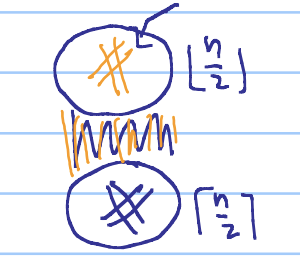
\includegraphics[width=0.3\textwidth]{non-induced-m2}
  \end{center}
  Then, $E(G_1) \cap E(G_2)$ is triangle-free and
  \begin{align*}
    e(G_1) + e(G_2) 
    &= 2e(G_1 \cap G_2) + e(G_1 \Delta G_2) \\
    &= 2\left\lfloor\frac{n^2}{4}\right\rfloor + \binom{n}{2} - \left\lfloor\frac{n^2}{4}\right\rfloor = \binom{n}{2} + \left\lfloor\frac{n^2}{4}\right\rfloor.
  \end{align*}

  Here we introduce the notation of \textit{compression} of $G_1, \ldots, G_m$, which is the graph
  obtained by moving all edges in only one $G_i$ to $G_1$. Performing compression for the case $m =
  2$, we get 
  \[
    e(G_1) + e(G_2) = e(G_1) + e(G_1 \cap G_2) \leq \binom{n}{2} + \left\lfloor\frac{n^2}{4}\right\rfloor,
  \]
  with equality if and only if $G_1 = K_n$ and $G_2 = G_1 \cap G_2 =
  K_{\left\lceil\frac{n}{2}\right\rceil, \left\lfloor\frac{n}{2}\right\rfloor}$. That is, the
  extremal graphs for $m = 2$ are isomorphic, up to compression.

  We use the notion of compression to solve for $m = 3, 4$:
  \begin{theorem}
    Suppose that $E(G_i) \cap E(G_j)$ does not include $K_3$ for distinct $i, j$. Then,
    \[
      e(G_1) + e(G_2) + e(G_3) \leq \binom{n}{2} + 2\left\lfloor\frac{n^2}{4}\right\rfloor,
    \]
    with equality if and only if $G_1 = K_n$ and $G_2, G_3 = K_{\left\lceil\frac{n}{2}\right\rceil,
    \left\lfloor\frac{n}{2}\right\rfloor}$ after compression.
  \end{theorem}

  \begin{proof}
    Compressing $G_1, G_2, G_3$ yields
    \begin{align*}
      e(G_1) + e(G_2) + e(G_3) 
      &= e(G_1) + e(G_1 \cap G_2) + e(G_1 \cap G_3) \\
      &\qquad\qquad + 2[e(G_2 \cap G_3) - e(G_1 \cap G_2 \cap G_3)] \\
      &\leq \textcolor{red}{e(G_1) + e(G_1 \cap G_2) + e(G_1 \cap G_3) \quad \text{(should be lowerbound)}} \\
      &\leq \binom{n}{2} + 2\left\lfloor\frac{n^2}{4}\right\rfloor,
    \end{align*}
    with equality if and only if $G_1 = K_n$ and $G_1 \cap G_2, G_1 \cap G_3 =
    K_{\left\lceil\frac{n}{2}\right\rceil, \left\lfloor\frac{n}{2}\right\rfloor}$. The result now
    follows.
  \end{proof}

  \textcolor{red}{TODO: solve $m = 4$.}

  % \begin{theorem}
  %   Suppose that $E(G_i) \cap E(G_j)$ does not include $K_3$ for distinct $i, j$. Then,
  %   \[
  %     \sum_{i = 1}^4 e(G_i) \leq \binom{n}{2} + 3\left\lfloor\frac{n^2}{4}\right\rfloor,
  %   \]
  %   with equality if and only if $G_1 = K_n$ and $G_i = K_{\left\lceil\frac{n}{2}\right\rceil,
  %   \left\lfloor\frac{n}{2}\right\rfloor}$ for $i > 1$ after compression.
  % \end{theorem}

  % \begin{proof}
  %   Compress $G_1, \ldots, G_m$. Put $m + 1 = 1$. By inclusion-exclusion,
  %   \begin{align*}
  %     e(G_i)
  %     &= \sum_{j \neq i} e(G_i \cap G_j) - \sum_{\substack{j, k \neq i \\ k > j}} e(G_i \cap G_j \cap G_k) + e(G_1 \cap G_2 \cap G_3 \cap G_4) \\
  %     &= \sum_{j \neq i} [e(G_i \cap G_j) - e(G_i \cap G_j)]
  %   \end{align*}
  %   for $i > 1$. Hence,
  %   \[
  %     \sum_{i = 1}^4 e(G_i) = e(G_1) + \sum_{i = 2}^{m}\sum_{k = 2}^{4} (-1)^{k}\sum_{\substack{I \subseteq [m] \\ i \in I, |I| = k}} e\left(\bigcap_{j \in I} G_j\right)
  %   \]
  % \end{proof}
\end{document}